\documentclass[tikz, border=1mm]{standalone}

\usepackage{pgfplots}
\pgfplotsset{compat=1.15}
\usepackage{mathrsfs}
\usetikzlibrary{arrows}
\pagestyle{empty}


\begin{document}

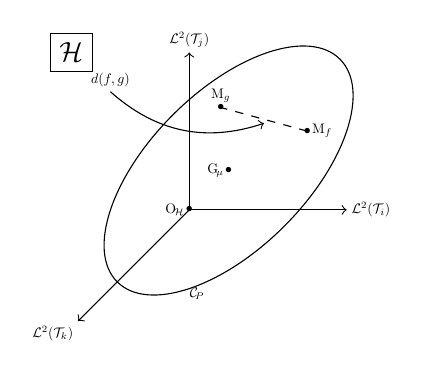
\begin{tikzpicture}

% Write
\node[draw] at (-1.5, 2) {$\mathcal{H}$};

% Axis
\draw[->] (0, 0) -- (2, 0);
\draw (2, 0) node[right, scale=0.5] {$\mathcal{L}^2(\mathcal{T}_i)$};

\draw[->] (0, 0) -- (0, 2);
\draw (0, 2) node[above, scale=0.5] {$\mathcal{L}^2(\mathcal{T}_j)$};

\draw[->] (0, 0) -- (-1.412, -1.412);
\draw (-1.412, -1.412) node[below left, scale=0.5] {$\mathcal{L}^2(\mathcal{T}_k)$};

% Points
\draw (0, 0) node[scale=0.5] {$\bullet$};
\draw (0, 0) node[left, scale=0.5] {$\mathrm{O}_{\!\mathcal{H}}$};

\draw (0.5, 0.5) node[scale=0.5] {$\bullet$};
\draw (0.5, 0.5) node[left, scale=0.5] {$\mathrm{G}_{\!\mu}$};

\draw (1.5, 1) node[scale=0.5] {$\bullet$};
\draw (1.5, 1) node[right, scale=0.5] {$\mathrm{M}_f$};

\draw (0.4, 1.3) node[scale=0.5] {$\bullet$};
\draw (0.4, 1.3) node[above, scale=0.5] {$\mathrm{M}_g$};

% Limes
\draw[dashed] (1.5, 1) -- (0.4, 1.3);

% Cloud
\draw[rotate around={45:(0.5, 0.5)}] (0.5, 0.5) ellipse (2cm and 1cm);
\draw (0.1, -1.2) node[above, scale=0.5] {$\mathcal{C}_{\!P}$};

% Distance
\draw (-1, 1.5) node[above, scale=0.5] {$d(f, g)$};
\draw[->] (-1, 1.5) to[bend right] (0.95, 1.1);

\end{tikzpicture}

\end{document}